\documentclass[nojss]{jss}
\usepackage{amsmath}
\usepackage{amssymb}

\title{\emph{em}: A Generic Function of the EM Algorithm for Finite Mixture Models in \proglang{R}}

\Plaintitle{em: A Generic Function of the EM Algorithm for Finite Mixture Models in R} 
\Shorttitle{em: the EM Algorithm in \proglang{R}}

\author{Dongjie Wu\\Københavns Universitet}
\Plainauthor{Dongjie Wu}

\Address{
  Dongjie Wu\\
  Sociologisk Institut \\ Københavns Universitet\\
  Øster Farimagsgade 5 \\ 1353 Copenhagen \\
  E-mail: \email{dongjie.wu@soc.ku.dk}
}

\usepackage[utf8]{inputenc}
\usepackage{listings}
\newcommand{\R}{\proglang{R}}
\lstset{frame=tb,
language=R,
keywordstyle=\color{blue},
alsoletter={.}
}


\Abstract{ 
  Our \emph{em} package follows \proglang{R}'s feature of generic functions and the function \code{em()} can be implemented after a model fitting with one component using R's pre-existing
functions and packages such as \code{glm()}, \code{lm()}, and so on.

Currently, it supports the following models: linear models (\code{lm()}), generalized linear models (\code{glm()}), generalized non-linear model (\code{gnm()}), survival models (mainly conditional logistic regression) (\code{survival::clogit()}), multinomial models(\code{nnet::multinom()}).
}

\Keywords{\proglang{R}, the EM Algorithm, finite mixture models, model based clustering, latent
  class regression}
\Plainkeywords{R, the EM Algorithm, finite mixture models, model based clustering, latent
  class regression}

%%\usepackage{Sweave} %% already provided by jss.cls
%%\VignetteIndexEntry{em: A Generic Function of the EM Algorithm for Finite Mixture Models in R}
%%\VignetteDepends{em}
%%\VignetteKeywords{R, the EM Algorithm, finite mixture models, model based clustering, latent class regression}
%%\VignettePackage{em}


\begin{document}

   \section{Introduction}
Finite mixture models (FMMs) are widely applied in both natural science and social science to model unobserved heterogeneity\footnote{See \citet{mclachlan2019finite} for an introduction of finite mixture models}. This modelling technique assumes that data can be divided into unobserved groups known as latent classes, each following a distinct probability density or a regression model with its unique model parameters. 

One reason for the extensive usage of finite mixture modelling is its flexibility. Its core assumption of unobserved heterogeneity can be applied on a variety of models and analysis including generalized linear regression models (GLMs), generalized non-linear regression models (GNMs), survival analysis, and etc. It can also be used as a model-based clustering technique with different data structures, for example, categorical data, multidimensional data and hierarchical data \citep{vermunt2008latent}. In addition, FMMs can parameterize probabilities of belonging to latent classes (i.e. a concomitant model \citep{wedel2002concomitant}) or extend FMMs to a nested or hierarchical structure \citep{vermunt2005hierarchical}.
% Flexibility and extension like Mixture of expert in Machine learning.
% Categorical variables 
% mixture of growth, etc.

% Introductioin of estimating FMM, Moment of Moment, MLE with EM and baysian types of measures.
In general, FMMs can be estimated by the following four methods: Methods of moments (MoM), Maximum log-likelihood estimation (MLE), the Bayesian methods, and the unsupervised machine learning methods \citep{Figue2002}. MLE using \emph{Expectation-maximization} (EM) algorithm is the mainstream method of estimating FMM models due to its performance and accuracy. However, it is relatively computationally intensive as it involves iteratively computing log-likelihood values. 

% Why we choose making this em package instead of using other packages.
% A bit of dicussions on packages available especially in R environments.
% And the generic function features.
There are many packages or software available for FMM models: e.g.  \emph{fmm} \citep{deb2007} and \emph{gllamm} \citep{rabe2004gllamm} in Stata, \emph{flexmix} \citep{leisch2004flexmix}, \emph{mixtools} \citep{benaglia2010mixtools} and \emph{mclust} \citep{scrucca2016mclust} in R, etc.
We make our own package \emph{em} for estimating FMM using EM because packages mentioned above did not cover the case for our own research. To provide a user-friendly package, we adopt a framework based on generic functions in R, which integrates better with other functions and packages in R and makes implementing FMM models more flexible and straightforward.

% Intro of following chapter.
In section 2, we specify FMMs and their extended variations. In section 3, we present EM algorithms and the approaches we use to fit FMMs. In section 4, we introduce the \emph{em} package and the generic \emph{em} function for fitting FMMs in R. Section 5 demonstrates some examples of using \emph{em}. Section 6 provides a short summary of the paper.   
   \section{Finite Mixture Models}
      \subsection{The Finite Mixture Models}
	      Finite mixture models can be described in the following equations given $J$ components:
      \begin{equation}
	      f(\mathbf{y}|\mathbf{x},\phi) = \sum_{j=1}^J \pi_j(f_j(\mathbf{y}|\mathbf{x}, \theta_j))
	    \end{equation}
	    where $\sum_{j=1}^J \pi_j = 1$,  $\mathbf{y}$ is a dependent variable with conditional density $f$,  $\mathbf{x}$ is a vector of independent variables, $\pi_j$ is the prior probability of component $j$,  $\theta_j$ is the component specific parameters for the density function $f_j$.

The model $f_j(\mathbf{y}|\mathbf{x}, \theta_j)$ can be one of a wide range of models: probability distributions, generalized linear models (GLM), generalized non-linear models (GNM),  survival models,  categorical models, etc. % TODO: introduction of a bunch of the models and the relavent R package.

Given the fitted model, one can compute the posterior probability that observation $i$ belongs to class $j$ using the following equation:
\begin{equation}
    Pr(j|\mathbf{x}, \phi, \mathbf{y}) = \pi_k\frac{f_k(\mathbf{y}|\mathbf{x}, \theta_j)}{\sum_{j=1}^J \pi_j(f_j(\mathbf{y}|\mathbf{x}, \theta_j))}
\end{equation}

The prior probability can also be parameterized by a vector of variables $\mathbf{z}$. In this case, a concomitant model is established in the following equation:
    \begin{equation}
      f(\mathbf{y}|\mathbf{x},\phi) = \sum_{j=1}^J \pi(\mathbf{z})(f_j(\mathbf{y}|\mathbf{x}, \theta_j)) \\
    \end{equation}
where $\pi(\mathbf{z})$ is a function that determines the prior probability by a vector of variables $\mathbf{z}$.
% TODO: Describe the model and its use on social science
      \subsection{The Hierarchical Mixture Models}
   \section{Fitting FMM using the EM Algorithm and its Extensions}
   EM algorithm is the mainstream approach to fitting finite mixture models. It runs iteratively through an expectation step (E-step) and a maximization step (M-step). Given an FMM, the E-step computes posterior probabilities given the estimation on last step, while the M-step estimates the model by maximizing the log-likelihood function.
   The log-likelihood function generated by an FMM can be rewritten in the following equation:
   \begin{equation}
   L_I(\theta|\mathbf{y},\mathbf{x}) = \sum_{i \in N} \log \sum_{j \in J} \pi_j f_j(y_i | x_i, \theta_j)
   \end{equation}
   An FMM can be treated as a model with missing data represented by latent classes. Therefore, we can assume a variable $w$ that captures which class each observation belongs to. In this case, the data $\{\mathbf{y}, w\}$ becomes a complete data. Base on this complete data, we can write the following complete-data log-likelihood function.
   \begin{equation}
      L_C(\theta|\mathbf{y},\mathbf{x}, w) = \sum_{i \in N} \log \sum_{j \in J} w_i \pi_j f_j(y_i| x_i, \theta_j)
   \end{equation}
   Since the EM is computational intensive due to its iterative nature, we provide two extensions of the EM algorithm in our package. One is the Categorical EM (CEM) and the other is the Stochastic EM (SEM). CEM assigns each observation to a certain class based on a higher posterior probability while SEM randomly assigns each observation to a certain class based on the observation's posterior probabilities for each class. 
   
   Using either CEM or SEM, we can assign each observation after an E-step, and estimate the model respectively for each class. This approach requires no fitting for a mixed version of log-likelihood functions. Therefore, it could be more computational efficient when the model is easier to fit given one class.
   
   However, this classification approach may not work well when a one-class model has a flat log-likelihood function such as a conditional logistics model. In this case, variations between class are hard to differentiate by an assignment of observations to each class. To fit this type of models, we adopt EM algorithm with a complete-data log-likelihood. A complete-data log-likelihood increases steepness of the log-likelihood function so that the EM algorithm can differentiate classes and search for the maximum. 
   
   To improve the performance of model-fitting, we make use of the \emph{Rcpp} and \emph{RcppArmadillo} packages to embed c++ code in R. When the computational process runs to maximize a log-likelihood function. The R programs make uses of the \code{optim} function in R to call the embed c++ code. In an E-step, we also use the c++ code to compute posterior probabilities. The use of c++ massively reduces the computational time of estimating a complete-data log-likelihood function and, therefore, improves the computational efficiency.    
   
   % Starting value
   For running EM algorithm, we also provide several methods to generate starting values. Starting values are crucial for fitting a mixture model as the log-likelihood function of a mixture model usually has several local optimums. Choosing a starting value deviated from the global optimum can lead to a less optimal result. In the package, we created two arguments \code{init.method} and \code{optim.start} for methods generating starting values. \code{init.method} generates the starting clustering for each observation. The available methods are: \code{random} -- a random assignment to a class, \code{kmeans} -- a k-mean clustering of data, and \code{hc} -- a model-based agglomerative hierarchical clustering. An m-step runs immediately after clustering to provide the starting values for the model parameters.
   
   If the complete log-likelihood function is using in the estimation, we use \code{optim.start} for generating the starting value of MLE. In the current version, it supports two methods: \code{random} generates a set of random values and \code{sample5} generates five sets of random values and run MLE with each set of random values for five times. Values with the largest log-likelihood are picked for the starting values of next round of MLE.  
   % methods recommandations.
   
   For simple models like generalized linear regression models, we recommend using \code{kmeans} or \code{random} to generate the staring values. For more complex models like a conditional logit model, fitting a complete log-likelihood function with the \code{sample5} start is necessary.
   
   \section{Using the Generic em Function}
   As a generic function, the \emph{em} function can take different models as its input. Currently, it supports the following models implemented in both the R base package and external packages:  linear models (\code{lm()}), generalized linear models (\code{glm()}),  generalized non-linear model (\code{gnm()}),  survival models (mainly conditional logistic regression) (\code{survival::clogit()}), multinomial models(\code{nnet::multinom()}).
   The following function describes the default \emph{em} function:
\begin{lstlisting}
em(object, latent=2, verbose=F, 
   init.method = c("random", "kmeans", "hc"),
   init.prob = NULL, algo= c("em", "cem", "sem"),
   cluster.by=NULL, max_iter=500, 
   abs_tol=1e-4, concomitant=list(...),
   use.optim=F, optim.start=c("random","sample5"), ...)
\end{lstlisting}
    where \code{object} is a model object such as \code{lm()} and \code{glm()}, \code{latent} determines the number of latent classes, \code{verbose} allows printing the fitting process, \code{init.method} provides three different initialization methods, \code{init.prob} allows users to determine the staring prior probabilities, \code{algo} provides three extensions of EM algorithms, \code{cluster.by} is the variable data is clustered by, \code{max_iter} determines the maximum steps for iteration, \code{abs_tol} is the absolute tolerance -- the difference between two log-likelihood values, \code{concomitant} allows users to set a concomitant model, \code{use.optim} decides whether to use the function \code{optim()} to maximize log-likelihood functions, and \code{optim.start} determines the method to generate the starting values for \code{optim()}.\footnote{For more detail, please check \emph{em} documentations.}
   \section{Examples}
   \subsection{Mixture of Generalized Linear Models}
   In the first example, we mix two linear models described in the following two equations with probabilities 30\% and 70\% respectively:
   \begin{eqnarray}
   y &=& {-10} + 0.1 x \\
   y &=& 20 - 0.1 x
   \end{eqnarray}
  The models can be fitted and presented using the following lines of codes in \proglang{R}.
\begin{Schunk}
\begin{Sinput}
R> library("em")
R> data("simreg")
R> fit.lm <- lm(yn~x, data=simreg)
R> summary(fit.lm)
\end{Sinput}
\begin{Soutput}
Call:
lm(formula = yn ~ x, data = simreg)

Residuals:
    Min      1Q  Median      3Q     Max 
-25.720 -18.166   7.212   9.926  17.206 

Coefficients:
            Estimate Std. Error t value Pr(>|t|)    
(Intercept) 10.73792    1.22736   8.749   <2e-16 ***
x           -0.04715    0.18710  -0.252    0.801    
---
Signif. codes:  0 '***' 0.001 '**' 0.01 '*' 0.05 '.' 0.1 ' ' 1

Residual standard error: 13.59 on 998 degrees of freedom
Multiple R-squared:  6.362e-05,	Adjusted R-squared:  -0.0009383 
F-statistic: 0.0635 on 1 and 998 DF,  p-value: 0.8011
\end{Soutput}
\begin{Sinput}
R> results <- em(fit.lm, latent=2, verbose=F)
R> summary(results)
\end{Sinput}
\begin{Soutput}
Call:
em.default(object = fit.lm, latent = 2, verbose = F)

Coefficients: 
              Estimate Std. Error t value Pr(>|t|)    
1.(Intercept) -9.88442    0.18569 -53.230   <2e-16 ***
1.x            0.07305    0.02819   2.591   0.0097 ** 
2.(Intercept) 19.74555    0.25442  77.611   <2e-16 ***
2.x           -0.05942    0.03886  -1.529   0.1265    
---
Signif. codes:  0 '***' 0.001 '**' 0.01 '*' 0.05 '.' 0.1 ' ' 1

Prior Probabilities: 
Comp.1: 0.31
Comp.2: 0.69


logLik: -2975, AIC: 5964, BIC: 5999. 
\end{Soutput}
\end{Schunk}
  In the code block showing above, we use \code{summary()} to print and summarize results after the use of \code{em()}. We organize the presentation of results in a similar look comparing with the summary of an baseline one-class model (like \code{lm()}). The difference is that we add a prefix $1.$ or $2.$ to represent which class the coefficients belong to. In addition, we present prior probabilities below the table of coefficients to show the proportion of each class in the mixture model.
  
  The summary of \code{em} fitting shows that the results are close enough to the true values. After the model fitting, we can use other generic functions in R for post-estimations and results printing. The supporting generic functions in the current version are as follows: \code{summary()}, \code{print()}, \code{predict()}, \code{update()}, \code{logLik()},\code{df()}, \code{plot()}.   

\begin{Schunk}
\begin{Sinput}
R> fmm_fit <- predict(results)
R> str(fmm_fit)
\end{Sinput}
\begin{Soutput}
List of 3
 $ components:List of 2
  ..$ : Named num [1:1000] -9.56 -9.59 -9.42 -9.71 -9.46 ...
  .. ..- attr(*, "names")= chr [1:1000] "1" "2" "3" "4" ...
  ..$ : Named num [1:1000] 19.5 19.5 19.4 19.6 19.4 ...
  .. ..- attr(*, "names")= chr [1:1000] "1" "2" "3" "4" ...
 $ mean      : num [1:1000, 1] 10.5 10.5 10.4 10.5 10.5 ...
 $ prob      : chr "prior"
 - attr(*, "class")= chr [1:3] "predict" "predict.em" "predict.prior"
\end{Soutput}
\begin{Sinput}
R> fmm_fit_post <- predict(results, prob="posterior")
R> str(fmm_fit_post)
\end{Sinput}
\begin{Soutput}
List of 3
 $ components:List of 2
  ..$ : Named num [1:1000] -9.56 -9.59 -9.42 -9.71 -9.46 ...
  .. ..- attr(*, "names")= chr [1:1000] "1" "2" "3" "4" ...
  ..$ : Named num [1:1000] 19.5 19.5 19.4 19.6 19.4 ...
  .. ..- attr(*, "names")= chr [1:1000] "1" "2" "3" "4" ...
 $ mean      : num [1:1000, 1:2] -3.84e-42 -8.02e-35 -8.03e-42 -1.02e-30 -5.12e-43 ...
 $ prob      : chr "posterior"
 - attr(*, "class")= chr [1:3] "predict" "predict.em" "predict.posterior"
\end{Soutput}
\end{Schunk}

In the above coding block, we use function \code{predict()} to predict values based on the results from the model fitting. In the default mode, \code{predict()} produces the fitted values for each component saved in the list \code{components} and computes the weighted mean based on the fitted values for each component and the prior probability $\pi$:
\begin{equation}
\hat{y} = \sum_{j \in J} \pi_j \hat{y_j} 
\end{equation}
The results for the weighted sum are saved in a vector \code{mean}. 

We can set the argument \code{prob="posterior"} to compute the fitted values weighted by the posterior probability using the following equation:
\begin{equation}
\hat{y} = \sum_{j \in J} \pi_{ij} \hat{y_j} 
\end{equation}
where $\pi_{ij}$ is the posterior probability. 

For data visualization, we use \code{plot()} to produce graphs after the model fitting \code{em()}. In the current version, \code{plot()} supports producing density plots by component and histograms of posterior probabilities. One can set up the figure using the argument \code{by}. 

% Graph (plot)
\begin{figure}[htp]
\caption{The counterfactual distribution of the predicted by component}
\label{fig:plot1}
\centering
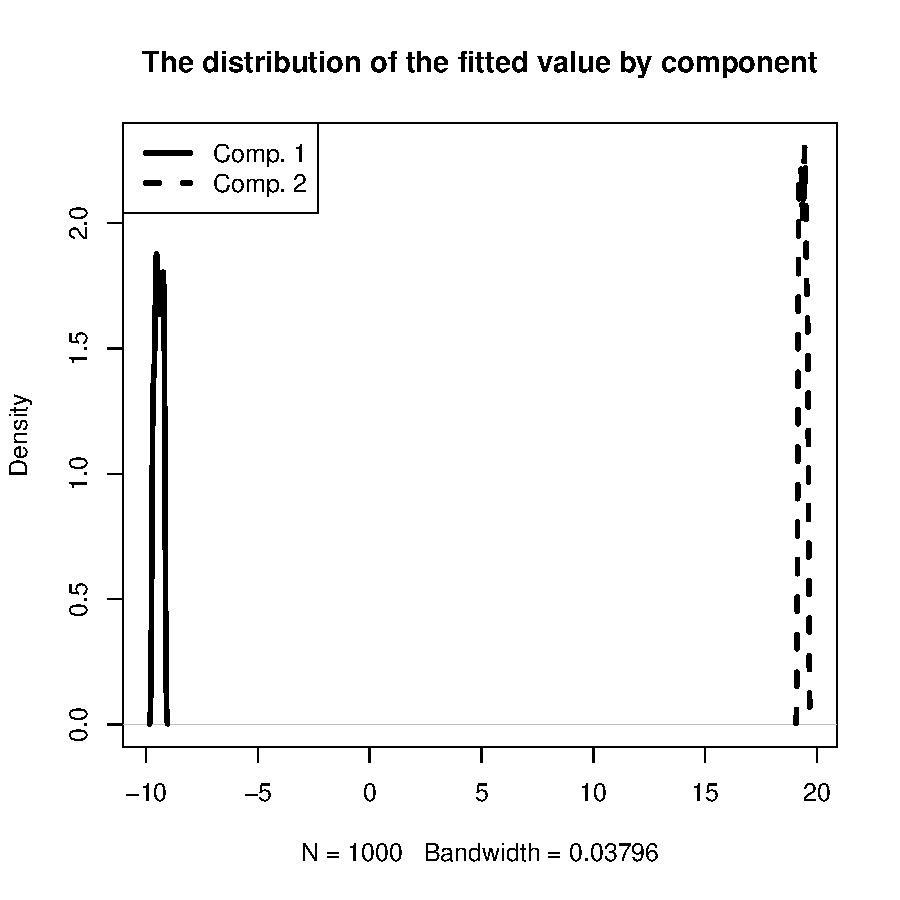
\includegraphics{em_intro-004}
\end{figure}
In the default mode, \code{plot()} produces a graph of distributions of the predicted for each component. Figure \ref{fig:plot1} is the demonstration. 

\begin{figure}[htp]
\caption{Histograms of posterior probabilities}
\label{fig:plot2}
\centering
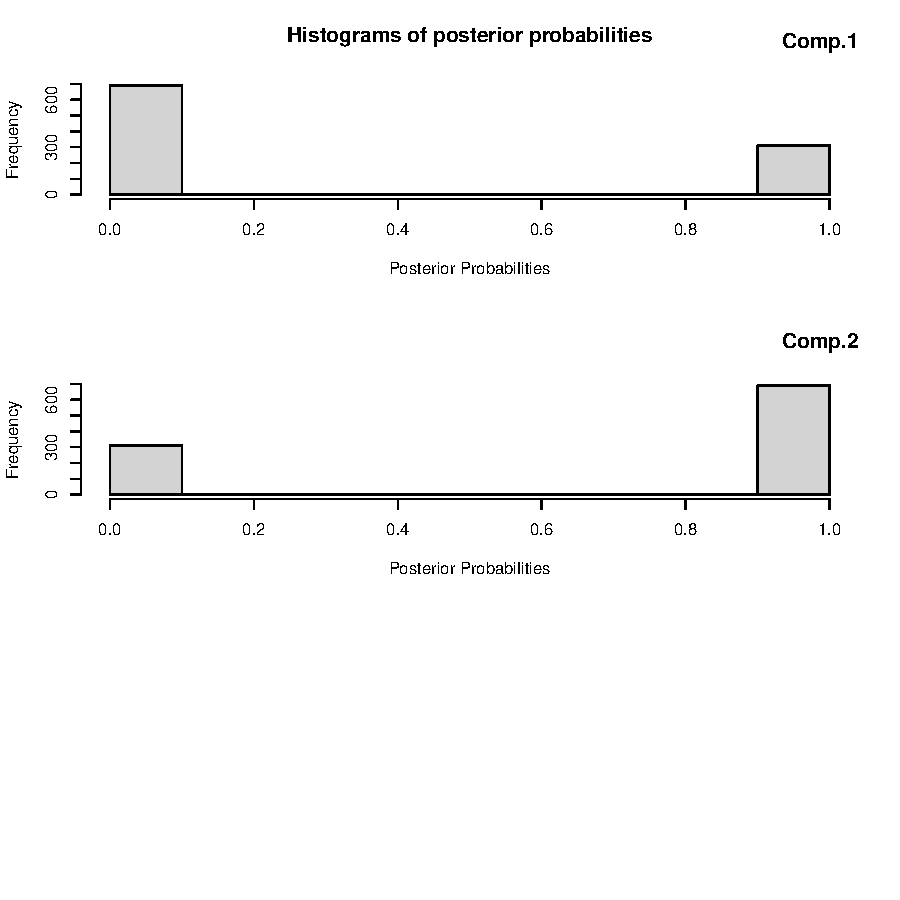
\includegraphics{em_intro-005}
\end{figure}

Figure \ref{fig:plot2} shows a histogram of posterior probability distributions.

We can also use a concomitant model to parameterize the prior probabilities. For example, we can assume the concomitant model in the following equations:
  \begin{eqnarray}
  y_c &=&  \pi_1(z) f_1(x) + \pi_2(z) f_2(x)\\
  \pi_1 + \pi_2 &=& 1 \\
  \pi(z) &=& g(z) 
  \end{eqnarray}

Given the equations, we run the following lines of codes:
\begin{Schunk}
\begin{Sinput}
R> formula <- yc ~ x
R> formula_c <- ~ z
R> lm_fit <- lm(formula, data=simreg)
R> results <- em(lm_fit, concomitant=list(formula=formula_c, data=simreg))
R> summary(results)
\end{Sinput}
\begin{Soutput}
Call:
em.default(object = lm_fit, concomitant = list(formula = formula_c, 
    data = simreg))

Coefficients: 
               Estimate Std. Error t value Pr(>|t|)    
1.(Intercept)  20.69606    0.26784  77.271  < 2e-16 ***
1.x            -0.23917    0.04072  -5.874 5.79e-09 ***
2.(Intercept) -10.13260    0.18380 -55.129  < 2e-16 ***
2.x             0.09922    0.02806   3.536 0.000424 ***
---
Signif. codes:  0 '***' 0.001 '**' 0.01 '*' 0.05 '.' 0.1 ' ' 1

Prior Probabilities: 
Comp.1: 0.339
Comp.2: 0.661

Concomitant model: 
              Estimate Std. Error t value Pr(>|t|)
2.(Intercept)   0.1843     0.1280   1.440    0.150
2.z            -0.2978     0.2233  -1.334    0.183

logLik: -2948, AIC: 5912, BIC: 5951. 
\end{Soutput}
\end{Schunk}
In the summary of results, we print the results from the concomitant model including the logistic regression of $\pi(z)$.

   \subsection{Mixture of Conditional Logistic Regression Models}
   In this example, A three-level outcome $y$ is generated by a mixture of two multinomial regressions with a three-level variable $x$ described in the following equations. \\
   Class 1: \\
   \begin{eqnarray}
   ln \frac{Pr(y_i = 2)}{Pr(y_i = 1)} &=& 2.1 x_2 + 4.1 x_3 \\
   ln \frac{Pr(y_i = 3)}{Pr(y_i = 1)} &=& 8.1 x_2 - 0.1 x_3
   \end{eqnarray}
   Class 2: \\
   \begin{eqnarray}
   ln \frac{Pr(y_i = 2)}{Pr(y_i = 1)} &=& 20.3 x_2 + 1.9 x_3 \\
   ln \frac{Pr(y_i = 3)}{Pr(y_i = 1)} &=& 10.5 x_2 + 0.7 x_3
   \end{eqnarray}   
   The probability of the mixture is 0.3 and 0.7 for two classes, respectively.
\begin{Schunk}
\begin{Sinput}
R> library("em")
R> library("survival")
R> data("simclogit")
R> fmla <- chosen2 ~ 0 + a2_x2 + a2_x3 + a3_x2 + a3_x3+ strata(id)
R> cfit <- clogit(fmla, simclogit)
R> emfit <- em(cfit, latent=2, verbose=F, init.method="kmeans", use.optim=T, optim.start="sample5", max_iter=100)
\end{Sinput}
\begin{Soutput}
Random start: 1
Iteration 1: (EM) log likelihood = 14323.5221
Iteration 2: (EM) log likelihood = 14033.9953
Iteration 3: (EM) log likelihood = 14004.4842
Iteration 4: (EM) log likelihood = 14001.2086
Iteration 5: (EM) log likelihood = 14000.8126
Random start: 2
Iteration 1: (EM) log likelihood = 14323.5221
Iteration 2: (EM) log likelihood = 13987.5831
Iteration 3: (EM) log likelihood = 13996.8977
Iteration 4: (EM) log likelihood = 14003.7911
Iteration 5: (EM) log likelihood = 14005.0099
Random start: 3
Iteration 1: (EM) log likelihood = 14323.5221
Iteration 2: (EM) log likelihood = 13814.0416
Iteration 3: (EM) log likelihood = 13767.1343
Iteration 4: (EM) log likelihood = 13761.0806
Iteration 5: (EM) log likelihood = 13760.0858
Random start: 4
Iteration 1: (EM) log likelihood = 14323.5221
Iteration 2: (EM) log likelihood = 14198.8056
Iteration 3: (EM) log likelihood = 14244.7413
Iteration 4: (EM) log likelihood = 14249.8756
Iteration 5: (EM) log likelihood = 14250.3362
Random start: 5
Iteration 1: (EM) log likelihood = 14323.5221
Iteration 2: (EM) log likelihood = 14474.4036
Iteration 3: (EM) log likelihood = 14471.6073
Iteration 4: (EM) log likelihood = 14471.5818
Iteration 5: (EM) log likelihood = 14471.6738
Iteration 0: (EM) log likelihood = 13759.9111
Iteration 1: (EM) log likelihood = 13759.5697
Iteration 2: (EM) log likelihood = 13759.5447
Iteration 3: (EM) log likelihood = 13759.5073
Iteration 4: (EM) log likelihood = 13759.5583
Iteration 5: (EM) log likelihood = 13759.5316
Iteration 6: (EM) log likelihood = 13759.529
Iteration 7: (EM) log likelihood = 13759.5186
Iteration 8: (EM) log likelihood = 13759.5082
Iteration 9: (EM) log likelihood = 13759.4992
Iteration 10: (EM) log likelihood = 13759.4988
Iteration 11: (EM) log likelihood = 13759.4959
Iteration 12: (EM) log likelihood = 13759.4972
Iteration 13: (EM) log likelihood = 13759.4948
Iteration 14: (EM) log likelihood = 13759.4951
Iteration 15: (EM) log likelihood = 13759.4945
Iteration 16: (EM) log likelihood = 13759.4948
Iteration 17: (EM) log likelihood = 13759.4942
Iteration 18: (EM) log likelihood = 13759.4946
Iteration 19: (EM) log likelihood = 13759.4951
Iteration 20: (EM) log likelihood = 13759.4959
Iteration 21: (EM) log likelihood = 13759.496
Iteration 22: (EM) log likelihood = 13759.4979
Iteration 23: (EM) log likelihood = 13759.4965
Iteration 24: (EM) log likelihood = 13759.4978
Iteration 25: (EM) log likelihood = 13759.498
Iteration 26: (EM) log likelihood = 13759.4987
Iteration 27: (EM) log likelihood = 13759.4987
\end{Soutput}
\begin{Sinput}
R> print(summary(emfit))
\end{Sinput}
\begin{Soutput}
Call:
NULL

Coefficients: 
             coef exp(coef)  se(coef)      z Pr(>|z|)    
1.a2_x2 7.261e+00 1.424e+03 1.000e+00  7.260 3.87e-13 ***
1.a2_x3 3.989e+00 5.398e+01 6.665e-02 59.846  < 2e-16 ***
1.a3_x2 6.753e+00 8.568e+02 1.001e+00  6.750 1.48e-11 ***
1.a3_x3 1.256e+00 3.513e+00 7.831e-02 16.044  < 2e-16 ***
2.a2_x2 1.084e+01 5.082e+04 1.000e+00 10.834  < 2e-16 ***
2.a2_x3 8.993e-01 2.458e+00 6.665e-02 13.494  < 2e-16 ***
2.a3_x2 8.904e+00 7.358e+03 1.001e+00  8.899  < 2e-16 ***
2.a3_x3 5.079e-01 1.662e+00 7.831e-02  6.486 8.84e-11 ***
---
Signif. codes:  0 '***' 0.001 '**' 0.01 '*' 0.05 '.' 0.1 ' ' 1

Prior Probabilities: 
Comp.1: 0.6721
Comp.2: 0.3279


logLik: -7954, AIC: 15927, BIC: 15992. 
\end{Soutput}
\end{Schunk}

Using the above code block, we make use of the function \code{clogit()} in the \code{survival} package and fit an FMM with two latent classes. We set \code{use.optim} to \code{TRUE} so that the \code{optim()} function is used with the embedded c++ code. To generate a start value for the M-step, we produce a set of random values for the parameters for five times. For each set of random values, we run the maximum log-likelihood estimate for five steps. We pick the values with the largest log-likelihood as the starting value.

The results are well-separated given two classes though they are not exactly the true values. 
   \section{Summary}
   The main challenge for implementing the EM algorithm and finite mixture modelling is that one could apply the mixture framework on any model. It could take immense effort and work if all models need to be built in the mixture form. In the \emph{em} package, we make use of the feature of generic functions in \proglang{R} so that our \code{em} function can attach to other available statistical models in \proglang{R}. Our package can, therefore, focus on algorithm development, results presentation and post-estimations.
   
   The current version of \code{em} supports most of generalized linear regressions implemented by function \code{lm} and \code{glm} in R. It also supports generalized non-linear regressions (\code{gnm}), multinomial regression models (\code{nnet::multinom}) and survival models (\code{survival::clogit}). Other models we are working on include mixture effect models (the \code{lme4} package) and mixture of distributions (the \code{fitdistrplus} package) and regressions with panel data (the \code{plm} package).
   
   When fitting a finite mixture model, many factors (such as starting values, algorithms and models we mixed) can determine whether the maximum log-likelihood value can be converged. The \code{em} package provides several extensions of EM algorithms and different methods to generate starting values for fitting. In addition, we provide a completed-data log-likelihood function for cases when a normal log-likelihood function is too flat. For estimating a completed-data log-likelihood function, we built a c++ module for speeding up the maximizing procedure so that a log-likelihood value is computed in c++ for each iteration. The c++ module massively reduces the computational time for the maximization part of the EM algorithm. For extensibility, These algorithms and methods are written independently in functions and objects so that more methods can be developed and included conveniently if necessary. 
   
   \section*{Acknowledgments}
   The research leading to the results presented in this article has received funding from the European Research Council (ERC) under the European Union’s Horizon 2020 research and innovation programme (grant agreement no. 851293). I am thankful to Dr. Kristian Bernt Karlson for his professional guidance and valuable advice. 
   \bibliography{em}
\end{document}
